\scanpage{30}
$F$ facette, alors \deleted{$\unsure{F}$} a) $F=\mathrm{int}_{A_F=A_{\overline F}}\overline F$, $\overline F=A_F\cap C=$

\deleted{b) $\overline F$ \unsure{est une} facette,}

b) $F'\subset C$ alors
\[
\begin{aligned}
&\underbrace{F'\ \text{facette de }\overline F}\\
&\hspace{3em}\unsure{\Updownarrow|\Downarrow}\\
&F'\ \text{facette de }C,\ F'\subset F
\end{aligned}
\]
[$\Rightarrow\overline F$ réunion de facettes]

c) Soit \deleted{$F$} $K\subset C$. Pour que $K$ soit \unsure{une} facette
fermée, il f. et S. que $K$ soit convexe, fermé et
une réunion de facettes. ($\Rightarrow$ une intersection
de deux facettes est une facette)

d) \deleted{\unsure{$L$}} Soit $\mathrm{Fac}(C)=\Pi$ \inserted{\unsure{l'ens|l'ens.} ordonné des facettes}. Alors

1°) $\Pi^\circ$ (l'ens. ordonné opposé) est isomorphe
à un ens $\unsure{\mathrm{Fac}'|\mathrm{Fac}}(C')$, où $C'$ est une
\inserted{\unsure{part. polyédriq|partie polyédriq|partie polyédrale}} convexe \deleted{\unsure{fermé}} dans $E$ de $=$ dim.

2°) \deleted{Soient} $F'_{\deleted{\unsure{1}}},F''_{\deleted{\unsure{2}}}\in\Pi$ \inserted{avec $F'<F''$}, $\Pi_{F',F''}$ l'ens ordonné des $F\in\Pi$, tels que $F'\leq \deleted{\unsure{F'}}F\leq F''$. Alors $\Pi_F$
est \inserted{$\simeq$ à un ens ordonné} de la forme \deleted{$\unsure{F}$} $\mathrm{Fac}(K')$, où
$K'$ un \inserted{polyèdre} convexe de dim $\delta=\dim F''-\dim F'-1$

% Short vertical emphasis stroke beside the corollary.
\uline{Cor} Si \deleted{\unsure{on}} $\dim F''-\dim F'=2$, alors \deleted{card} l'ens
des $F$ tels que $F'<F<F''$ est de card. $2$.

\figure{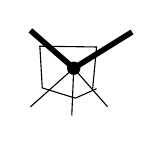
\begin{tikzpicture}[x=1cm,y=1cm]
\draw (-.44,.28)--(.29,.27)--(.24,-.26) (-.43,.27)--(-.4,-.25)--(.02,-.38)--(.29,-.26);
\draw (-.55,-.49)--(0,0)--(.43,-.49) (0,0)--(-.025,-.60);
\draw[line width=2pt] (-.55,.48)--(0,0)--(.74,.46);
\fill (0,0) circle (.085);
\end{tikzpicture}}

\uline{Polyèdre combinatoire} : ens ordonné
fini $I$ satisfaisant les conditions

a) $I$ a des inf et des sup \unsure{quelc}
[plus petit et plus gd élément, et
$i\wedge j$ et $i\vee j$]

b) $I$ satisfait condition des chaines

c) Si $i<j<$\deleted{\unsure{$d$}}$k$ et si $j$ succ. \deleted{\unsure{imméd.|immédiat}} de $i$
$k$ succ. de $j$
% archive sheet number: 29
